
MC samples of the aQGC signal processes described in \sec\ref{sec:eft}
have been generated using \vbfnlo at NLO in QCD.  (but don't we use LO?)
The cross-sections for the aQGC signal depend on the values
of the couplings $f_{s,0}$ and $f_{s,1}$. MC samples have 
been generated for a grid of points in the $f_{s,0}$ vs $f_{s,1}$ space
and their cross-sections are shown in \fig\ref{fig:aqgc_total_xsec_ununitarized_3l}. %histogram of cross-sections

\begin{figure}[ht!]
\centering
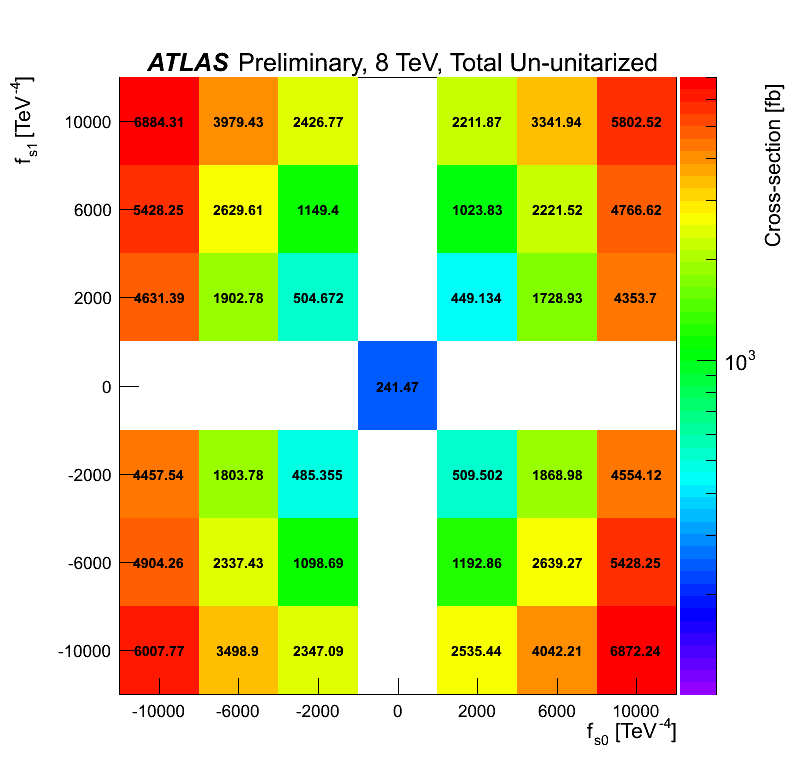
\includegraphics[width=.8\textwidth]{figures/aQGC/total_xsec/www_3l_aqgc_total_ununitarized_noratio.png}
\caption{Total cross-section for non-unitarized aQGC signal samples as a function of $f_{s,0}$ vs $f_{s,1}$.
The total SM cross-section is shown at $f_{s,0}=f_{s,1}=0$ for comparison.}
\label{fig:aqgc_total_xsec_ununitarized_3l}
\end{figure}

The issues of unitarity violation \sec\ref{sec:eft} are taken
into account using a form factor like in \eqn\eqref{eq:form_factor}.
The choices of the exponent, $n$, and form factor scale, $\Lambda$, 
are somewhat ad-hoc. Furthermore, a complete study of the unitarity
behavior of this process has never been performed, so there are not
currently detailed prescriptions on what to choose. 
However, based on discussions with the authors of \vbfnlo, who
are at the moment trying to perform these studies, an exponent
of $n=1$ is expected to be sufficient to acheive unitarity 
for this process.  As for the choice of $\Lambda$, we have
chosen to look at a few different values, which cover a wide
range but which should follow a smooth interpolation. 
This has the advantage of providing information about the
sensitivity to the form factor that can be interpreted 
by theorists as they see fit. Dedicated MC samples
are generated with the unitarization applied for values
of $\Lambda =$ 500~\GeV, 1000~\GeV, 2000~\GeV, and 3000~\GeV.
The cross-sections for each of these unitarization cases
are shown in \fig\ref{fig:aqgc_total_xsec_unitarized_3l}.

\begin{figure}[ht!]
\centering
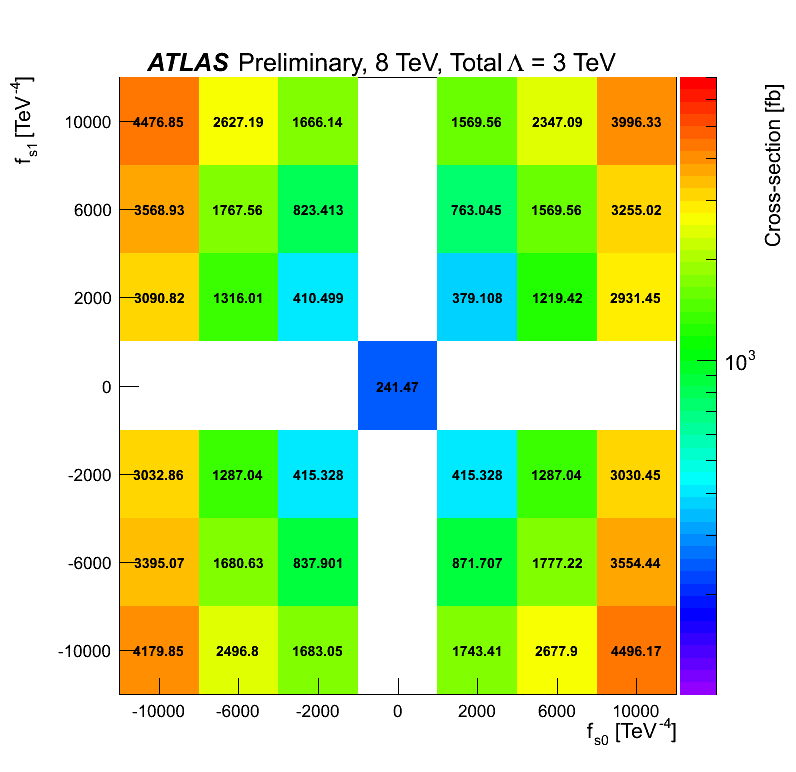
\includegraphics[width=.45\textwidth]{figures/aQGC/total_xsec/www_3l_aqgc_total_3TeV_noratio.png}
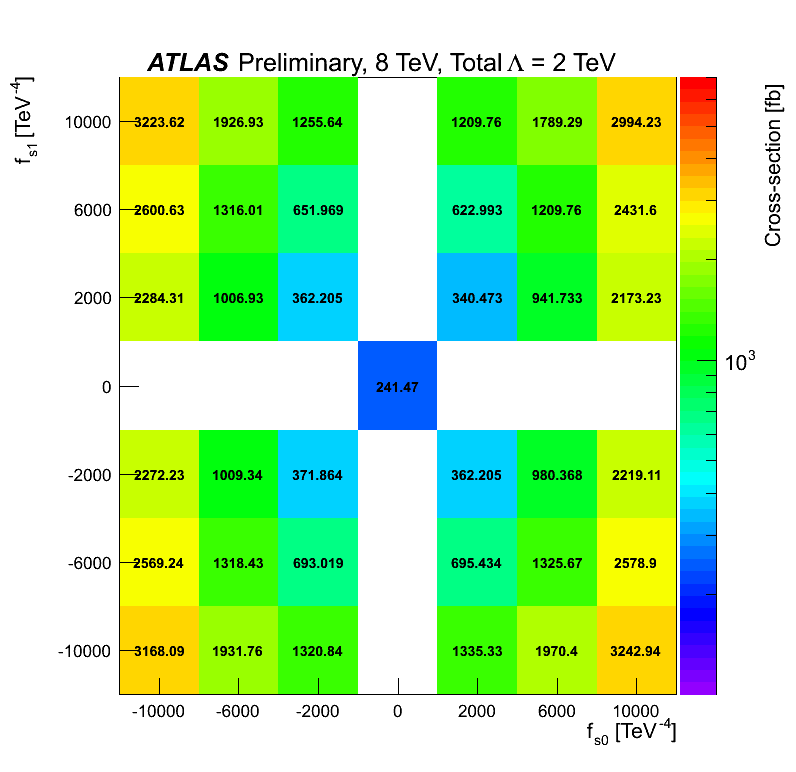
\includegraphics[width=.45\textwidth]{figures/aQGC/total_xsec/www_3l_aqgc_total_2TeV_noratio.png}
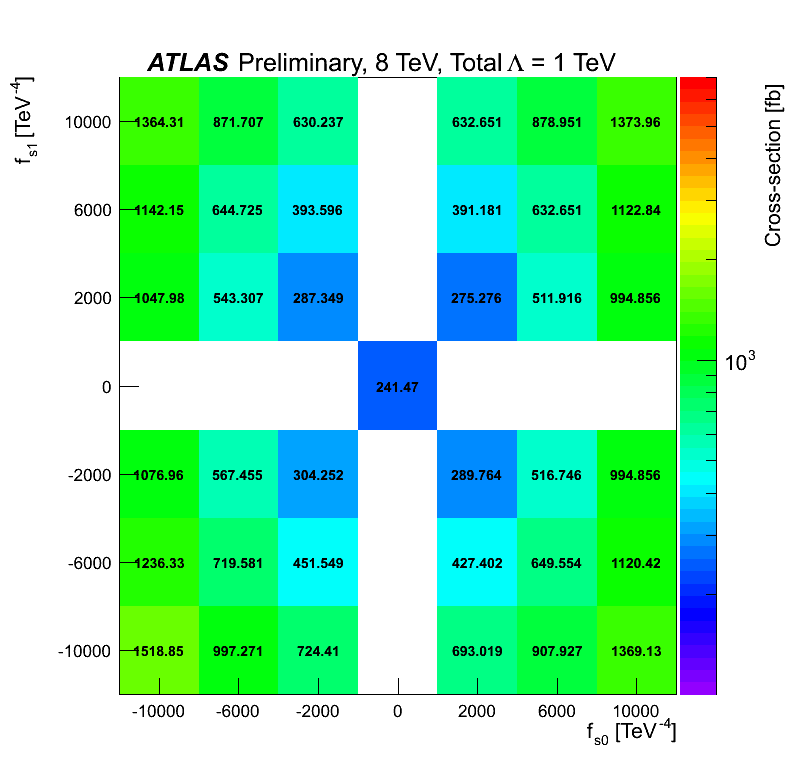
\includegraphics[width=.45\textwidth]{figures/aQGC/total_xsec/www_3l_aqgc_total_1TeV_noratio.png}
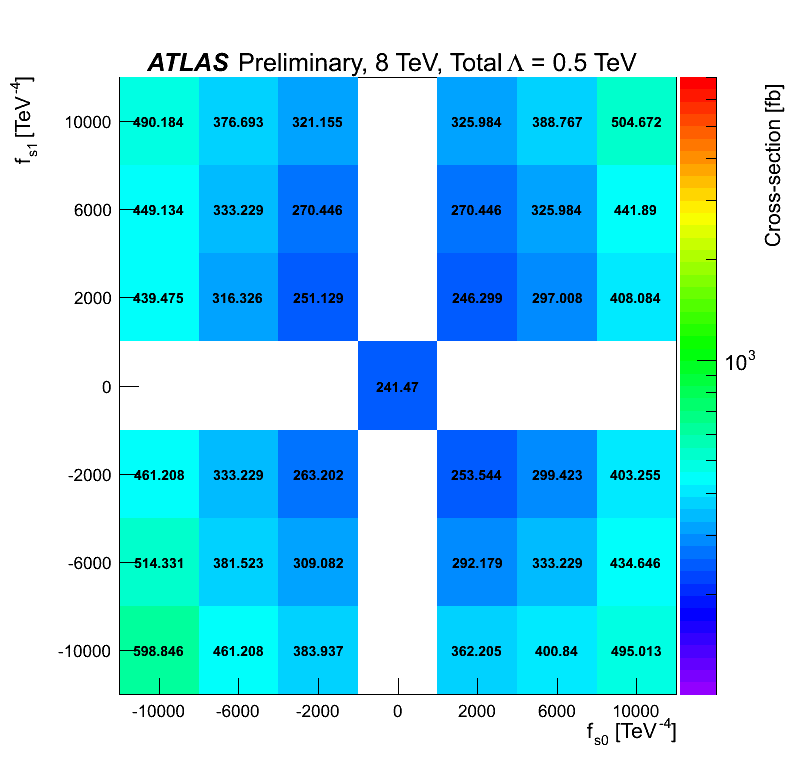
\includegraphics[width=.45\textwidth]{figures/aQGC/total_xsec/www_3l_aqgc_total_p5TeV_noratio.png}
\caption{Total cross-section for unitarized aQGC signal samples as a function of $f_{s,0}$ vs $f_{s,1}$.
Four different values of the unitarization scale, $\Lambda$, are chosen: 3~\TeV~(Top Left),
2~\TeV~(Top Right), 1~\TeV~(Bottom Left), and 0.5~\TeV~(Bottom Right).
The total SM cross-section is shown at $f_{s,0}=f_{s,1}=0$ for comparison.}
\label{fig:aqgc_total_xsec_unitarized_3l}
\end{figure}

